\documentclass[12pt,a4paper]{report}

\usepackage[english,frenchb]{babel}
\usepackage[T1]{fontenc}
\usepackage[utf8x]{inputenc}
\usepackage{fontspec}

\usepackage{lmodern}
\usepackage{fancyhdr}
\usepackage[colorlinks=true,urlcolor=blue]{hyperref}
\usepackage{xcolor,colortbl}
\usepackage{geometry}
\usepackage{multirow}
\usepackage{fancyvrb}
\usepackage{wrapfig}
\usepackage{graphicx}
\usepackage{tikz}
\usepackage{amsfonts}
\usepackage{amsmath}
\usepackage{amsthm}
\usepackage{floatrow}
\floatsetup[table]{capposition=top}
\renewcommand{\arraystretch}{1.5}

\makeatletter

\newcommand\frontmatter{%
	\cleardoublepage
	%\@mainmatterfalse
	\pagenumbering{roman}}

\newcommand\mainmatter{%
	\cleardoublepage
	% \@mainmattertrue
	\pagenumbering{arabic}}

\newcommand\backmatter{%
	\if@openright
	\cleardoublepage
	\else
	\clearpage
	\fi
	% \@mainmatterfalse
}

\makeatother

\renewcommand*{\FrenchLabelItem}{$\bullet$}



\begin{document}
	\frontmatter
	%\interfootnotelinepenalty=10000
	%\setlength{\headheight}{15.2pt}
	\pagestyle{fancy}
	\fancyhf{}
	\fancyhf[HR]{\thepage}
	\fancyhf[HL]{\leftmark}
	\hyphenation{}
	
	\newgeometry{top=2cm,bottom=1cm}
	
	%=============page de garde==============================
	\begin{titlepage}
		
		\begin{center}


		\begin{minipage}{0.5\textwidth}

		\begin{flushleft}
		
\includegraphics[width=4cm,height=3.2cm]{graphics/ensias.png}\\
		\begin{flushleft}
		 { \scriptsize  \'Ecole Nationale Supérieure \\[0.2cm]d’Informatique et d’Analyse\\ \hspace{10mm}des Systèmes  }

		\end{flushleft}

		 

		\end{flushleft}

		\end{minipage}
		\begin{minipage}{0.4\textwidth}
		\begin{flushright}
		
\includegraphics[width=4cm,height=3.2cm]{graphics/logo_softcentre.png}\\
		%{ \scriptsize  Facult\'e des Sciences Juridiques, \\ \'Economiques et Sociales - Oujda  }
		\end{flushright}

		\end{minipage}\\[3cm]



		{\normalsize Ingénierie web et informatique mobile }\\[0.5cm]

		{\normalsize M\'emoire de Stage de  1\up{er} Ann\'ee}\\[0.5cm]

		% Title
		\rule{\linewidth}{0.5mm} \\[0.4cm]
		%{ \large \bfseries Application mobile pour la réservation de véhicule sous la plateforme ScreenDy \\[0.4cm] }
		{ \large \bfseries Création d'une application mobile sous la plateforme ScreenDy \\[0.4cm] }
		\rule{\linewidth}{0.5mm} \\[3cm]

		% Author and supervisor
		\noindent
		\begin{minipage}{0.4\textwidth}
		  \begin{flushleft} \small
		    \emph{Réalisé par :}\\
		     Aymen \textsc{CHLA}\\
		  \end{flushleft}
		\end{minipage}%
		\begin{minipage}{0.4\textwidth}
		  \begin{flushright} \small
		    \emph{Encadré par :} \\
		    Mme.~Imane \textsc{BELLA}\\  
		  \end{flushright}
		\end{minipage}\\[4cm]

		\vfill

		% Bottom of the page
		{\large \slshape 24 Juillet - 31 Août 2017}

		\end{center}
	\end{titlepage}
	%=======================fin page de garde====================
	
	\restoregeometry
	\normalsize
	\clearpage
	\mainmatter


	%============blank  page==========
	\begingroup
	  \pagestyle{empty}
	  \null
	  \newpage
	\endgroup
	%============fin blank page==========
	
	
	

	%=============remerciement==============
	\chapter*{Remerciements}
	\addcontentsline{toc}{chapter}{Remerciements}
	
	Tout d'abord, je tiens à exprimer mes vifs remerciements et ma profonde gratitude à toute personne ayant contribué, de près ou de loin, à la réalisation de ce projet et ayant fait de cette période de stage un moment très profitable.\\
	\newline
	Je tiens particulièrement à remercier mon encadrante, Mme. Imane \bsc{BELLA}, pour son guide et ses conseils, ainsi que pour son encadrement durant toutes les phases de réalisation de ce projet.\\
	\newline
	Je tiens à exprimer les purs sentiments de reconnaissance et de sincères remerciements à ma famille, qui ma soutenus moralement durant cette période de stage qui ont favorisé son aboutissement.
	%===========fin remerciement============





	%===========résumer ====================
	\chapter*{Résumé}
	\addcontentsline{toc}{chapter}{Résumé}
	Le sujet de mon projet de stage, vise à développer une application mobile pour la réservation de véhicules basée sur la géolocalisation pour le compte de l'entreprise client du SOFT CENTRE: Screendy. Le travail s’est déroulé en plusieurs phases : Une phase d’analyse et de conception et une phase de développement.\\
Cependant, pour aboutir à cette fin, je vais tout d’abord effectuer une étude conceptuelle de l’application. Cette dernière me permettra, en effet, d’accéder facilement à la réalisation de l’application en organisant les idées et en structurant le processus de codage suivant des diagrammes UML. L’application a été développée avec du \guillemotleft ScreenDy JavaScript \guillemotright et par diverses technologies tout en se basant sur une étude conceptuelle.\\
Le système de gestion de base de données choisi fut Firebase.\\
Une deuxième partie du stage consiste à utiliser des APIs sur des applications ScreenDy.\\
Mots clés : UML, ScreenDy JavaScript, Firebase.
	%=======================================


	%===========résumer====================
	\chapter*{Abstract}
	\addcontentsline{toc}{chapter}{Abstract}
	The subject of my internship project, aims to develop a mobile application for booking vehicles based on geolocation for the client company of SOFT CENTRE: Screendy. The work took place in several phases: An analysis and design phase and a development phase.
However, to achieve this end, I will first make a conceptual study of the application. The latter will allow me, in fact, easy access to the implementation of the application by organizing the ideas and structuring the coding process according to UML diagrams. The application has been developed using \guillemotleft ScreenDy JavaScript \guillemotright and by various technologies while being based on a conceptual study. \\
The database management system chosen was Firebase.\\
A second part of the internship is to use APIs on ScreenDy applications.\\
Keywords: UML, ScreenDy JavaScript, Firebase. 
	%=======================================


	%==========tables==========
	\listoffigures
	\tableofcontents
	%=========================

	%===========introduction générale================
	\chapter*{Introduction générale}
	\addcontentsline{toc}{chapter}{Introduction générale}
	Ce rapport présente le travail que j'ai réalisé dans le cadre du stage de fin de 1\up{ère} ann\'ee, ayant comme objectif la réalisation d'une application mobile pour la réservation de véhicules basée sur la géolocalisation ainsi que la mise en place de templates utilisant des APIs sous la plateforme ScreenDy.\\
	En effet, le travail demandé vise à développer une application mobile qui serait par la suite mise sur le marketplace de la plateforme pour faciliter la création d'application semblable aux futurs développeurs ScreenDy.\\
	Dans ce rapport, je vais également présenter toutes les étapes que j'ai suivi pour arriver à la conclusion finale. Tout d'abord, il est évident de commencer par la présentation de l'organisme et du projet, pour ensuite aborder la partie pratique où nous passerons de l’idée à l’implémentation du code. Pour au final vous présentez quelques aspects du résultat final afin de vous permettre de découvrir au mieux mon travail.\\
	%===========fin introduction générale==============
	

	
	




%=========================chapitre 1========================
	\chapter{Présentation de l'organisme}
	\section{Mission}
	\begin{wrapfigure} {r}{4cm}
	
\includegraphics[scale=0.5]{./graphics/logo_softcentre.png}
	\end{wrapfigure}
		Le Soft Centre, dont la Présidence est assurée par l’ANRT (www.anrt.ma), est un Centre de développement logiciel mis à disposition des opérateurs du secteur de l’Industrie des Technologies de l’Information ; dans le but de leur permettre de produire du logiciel innovant en faisant appel aux compétences universitaires de recherche appliquée au sein des Universités et Ecoles d’ingénieurs.

	
        \section{Domaines d’intervention}
          Le Business Model du Soft Centre repose à ce jour sur le développement de 3 domaines d'intervention:\\
	\begin{itemize}
		\item La \textbf{recherche appliquée et le développement logiciel;} à savoir la génération de projets de recherche et de développement logiciel \guillemotleft à la demande\guillemotright.
		\item Le \textbf{centre de services partagés,} via la mise à disposition de ressources mutualisées au profit des opérateurs du secteur des IT, dans le but de favoriser l'essor du tissudes PME dans certains secteurs logiciels.
		\item L'\textbf{Open Innovation}, via la mise en oeuvre de \textbf{programmes d'accélération technologiques, } co-organisés de concert avec donneurs d'ordres nationaux et à destination des startups locales.
	\end{itemize}

	%==============mode de fonctionnement
 	\section{Mode de fonctionnement}
 La chaîne de valeur repose sur la mise en oeuvre des processus suivants :\newline
 	\begin{itemize}
 		\item Identification et montage de dossiers R\&D dans le domaine du développement logiciel.
		\item Syndication des compétences (en termes de recherche appliquée) au sein des Ecoles d’Ingénieurs et Universités Marocaines (Chercheurs, doctorants, thésards, étudiants ingénieurs en complément des ressources permanentes du Soft Centre constituées de chefs de projet et d’ingénieurs experts). 
		\item Hébergement des équipes de recherche intégrées via 
la mise à disposition des infrastructures technologiques requises.
		\item Pilotage des projets de R\&D logiciel au service des demandeurs.
	\end{itemize}
	%====================================

	%==============membre du conseil d'administration
	\subsection{Membres du Conseil d'Administration}
 	\begin{itemize}
		\item Ministère du Commerce, de l’Industrie et des Nouvelles Technologies.
		\item Ministère de l’Economie et des Finances
		\item Ministère de l’Enseignement Supérieur et de la Recherche Scientifique
		\item Agence Nationale de Règlementation des Télécommunications
		\item Caisse de Dépôt et de Gestion
		\item Centre National pour la Recherche Scientifique et Technologique
		\item Fédération des Technologies de l’Information, des Télécommunications et de l’Offshoring
	\end{itemize}
	%=============================================

	\newpage

	%===========présentation de l'entreprise cliente
	\begin{wrapfigure} {r}{3cm}
	
\includegraphics[scale=0.5]{./graphics/logo_screendy.png}
	\end{wrapfigure}
	\subsection{L'entreprise cliente}
		\subsection{Présentation de l'entreprise}
ScreenDy est une entreprise marocaine créer en 2013 ayant pour but de procurer aux développeurs une plateforme mobile basée sur le cloud qui permet de créer des applications 100\% natives (Android et IOS), custom et mobiles optimisées, puis de les déployer sur Mobile, Tablet, TV connectée et autres nouvelles plateformes à l'avenir.\\
ScreenDy a plus de 10 000 utilisateurs à travers le monde, 2345 applications et un chiffre d'affaires d'environ 1 million de dollars, l'entreprise souhaite dans 3 ans d'arriver à 1 million d'utilisateurs et un chiffre d'affaires de 100 millions de dollars.\\
C'est dans ce cadre que ScreenDy à travers l'organisme SOFT CENTRE recrute des jeunes stagiaires développeurs ayant pour mission la création d'applications mobiles avec ScreenDy à fin d'enrichir le \guillemotleft marketplace \guillemotright de la plateforme à fin d'offrir une multitude d'applications variées prêtes à l'emploi comme étant une base de départ pour donner encore plus d'aisance aux développeurs à réaliser leurs applications dans un temps-record.
		\subsection{Prix populaires}
Parmis les prix les plus populaires que ScreenDy a gagnée ces dernières années:\\
		\newline
		\begin{minipage}{0.5\textwidth}

		\begin{flushleft}
		
\includegraphics[width=3.2cm,height=3.2cm]{graphics/10ww.png}\\
		\begin{flushleft}
		 { \scriptsize  \textbf{Finaliste} \\[0.2cm]Top 10 des startups dans le monde\\Get In the Ring Global 2014}

		\end{flushleft}

		 

		\end{flushleft}

		\end{minipage}
	\begin{minipage}{0.5\textwidth}

		\begin{flushleft}
		
\includegraphics[width=3.2cm,height=3.2cm]{graphics/mit.png}\\
		\begin{flushleft}
		 { \scriptsize  \textbf{Gagnant} \\[0.2cm]Top 3 des startups dans la région MENA\\MIT EF Award 2015}

		\end{flushleft}

		 

		\end{flushleft}

		\end{minipage}
		
\begin{minipage}{0.5\textwidth}

		\begin{flushleft}
		
\includegraphics[width=3.2cm,height=3.2cm]{graphics/startupconferance.png}\\
		\begin{flushleft}
		 { \scriptsize  \textbf{Finaliste} \\[0.2cm]Top 3 des startups Silicon Valley\\The Startup
Conference 2015}

		\end{flushleft}

		 

		\end{flushleft}

		\end{minipage}
\begin{minipage}{0.5\textwidth}

		\begin{flushleft}
		
\includegraphics[width=3.2cm,height=3.2cm]{graphics/pionnersFestival.png}\\
		\begin{flushleft}
		 { \scriptsize  \textbf{Finaliste} \\[0.2cm]Top 10 des startups dans le monde\\Pioneers Festival 2015}

		\end{flushleft}

		 

		\end{flushleft}

		\end{minipage}


	%=============================================
%=================fin du chapitre 1===========================================



	

%========================chapitre 2===============================================
		\chapter{Projet de stage}
		
		%========présentation du projet===============
		\section{Problèmatique}
L’évolution de la technologie des télécommunications a donné naissance à plusieurs services,
notamment le service de la géolocalisation. Ce dernier est souvent utilisé dans les applications
mobiles et qui peut être intégré dans la stratégie de marketing mobile en offrant diverses possibilités
de localisation et le positionnement dans diffèrent domaines et surtout celui de la gestion des
réservations des locations des véhicules. Cette facilité a encouragé plusieurs entreprises surtout celle
qui produit des applications basées sur la géolocalisation à exprimer un besoin pour une gestion
automatique de leurs différents modules.\\
Après une consultation de la liste des applications réalisées avec ScreenDy et celle en cours de développement il s'est avéré que ce type d'application n'était pas encore proposé d'où l'intérêt que j'ai eu envers ce type application.\\
C’est donc dans ce cadre que s’inscrit mon projet de stage de fin de 1\up{ère} ann\'ee visant à établir
une bonne analyse et conception pour la mise en place d’une première version de ce système.

		
		%=================objectif==================
		\section{Objectif}
Mon projet de stage consiste donc à développer une application qui permettra de donner
une flexibilité à la gestion des réservations des véhicules. L’objectif est de stocker les informations
liées aux réservations dans une base de données et de permettre aux utilisateurs de retrouver facilement les données dont ils auront besoin pour effectuer les réservations.\\
L’objectif sera également d’avoir une interface UI conviviale originale et différente par rapport aux autres applications développées avec ScreenDy et d’utiliser au mieux les outils limités dont dispose la plateforme pour mettre au point ce projet.\\
Mon projet a donc comme principal objectif l’automatisation du processus de réservations des
véhicules. Il porte sur l’analyse, la conception, le développement d’une application mobile utilisant
un service web pour la récupération des données nécessaires pour offrir aux clients un service de
réservation avec une meilleure performance, rapidité et disponibilité.\\

		%=================Parties prenantes=================
		\section{Parties prenantes}
			\begin{itemize}
				\item Les clients: Adulte ayant un permis de conduire.
				\item Les directeurs de location, quant à eux, peuvent gérer les voitures et les offres de location relatives à leurs agences.
				\item L'administrateur est le profil aux plus grands privilèges. C'est un super utilisateur ayant le droit d'effectuer toutes sortes d'opérations, notamment la gestion des utilisateurs.

			\end{itemize}
		


		%=============== Description de l'application=============
		\section{Déscription de l'application}
L’application gère la réservation de véhicule dans les agences de location. Elle permet aux clients de réserver des véhicules en consultant la liste des offres les plus proches de leurs emplacements. Ils pourront ainsi consulter les détails des offres ainsi que l’emplacement des agences.
L’application permet au directeur de location de gérer les offres de leurs agences. Elle gère aussi la partie administration en gérant les comptes des utilisateurs. 
Également, l’application permet l’identification de chaque personne, dépendamment de son profil, lui donne accès à des options différentes.



		%===============specification des besoins===========================
		\section{Spécification des besoins fonctionnels}
L’application devra regrouper toutes les fonctionnalités nécessaires pour :\\
				\begin{itemize}
					\item \textbf{La création des comptes:} Le client pourra créer un compte sur l'application 
					\item \textbf{L'authentification:} L’utilisateur devra pouvoir s’authentifier à travers un email et un mot de passe. Le système vérifie l’authentification.
					\item \textbf{La consultation des offres disponibles:} Le client pourra visualisé les offres de réservations disponible.
					\item \textbf{Consulter les détails d'un offre:} Le client pourra consulté les détails d'un offre à savoir la marque, les options du véhicule, condition d'utilisation...
					\item \textbf{trier les offres selons l'emplacement:} Les offres s'affichent selon la position du client par défaut si l'option de localisation est activée.
					\item \textbf{reserver une voiture:} Le client pourra réserver à travers cette application tout en donnant un délai de 24 heures avant l'annulation.
					\item \textbf{Annuler la réservation:} A tout moment le client peut annuler la réservation.
					\item \textbf{Consulter les réservations:} Le client pourra consulter ses réservations ainsi que le temps restant avant l'annulation.
					\item \textbf{Gestion des offres:} Le directeur de location pourra ajouter, modifier, consulter et supprimer les offres de son agence.
					\item \textbf{Gestion des réservations:} Le directeur de location poura ajouter, modifier, consulter et supprimer les réservations des clients de son agence.
					 
				\end{itemize}

		\section{Spécification des besoins non fonctionnels:}		
Ces besoins caractérisent le système. Il s’agit de définir un ensemble de critères essentiels
pour le bon fonctionnement de l’application. Ceux-ci peuvent être relatifs aux performances, à la
conception ou au matériel.\\
Nos principaux besoins non fonctionnels sont, alors :\\
			\begin{itemize}
				\item \textbf{Ergonomie:} L’interface doit être simple et utilisable sans prérequis.
				\item \textbf{Sécurité:} Les comptes des utilisateurs sont sécurisés par mot de passe.
				\item \textbf{Extensibilité:} L’application doit permettre l’ajout de nouvelles fonctionnalités.
ou la modification de celles existantes facilement.
				\end{itemize}


		%============conclusion========================
		\section{Conclusion}
Dans ce chapitre j'ai présenté le cadre général de mon projet en déterminant l’objectif principal du projet. J'ai dévoilé les exigences des besoins fonctionnels et non fonctionnels. Dans le chapitre suivant je vais reproduire les différents besoins cités précédemment sous forme de diagrammes UML.
%==================================fin chapitre 2====================================











%===============================chapitre 3===========================================
	\chapter{Conception fonctionnelle}

		
		%============introduction===================
		\section{Introduction}
Dans cette section, je vais reproduire les différents besoins sous la forme de diagrammes UML.\\
UML est un langage de modélisation graphique pour fournir une méthode normalisée pour visualiser la conception d'un système. Il est couramment utilisé en développement logiciel et en conception orientée objet.
		
		%===========vue fonctionnelle=============
		\section{Vue fonctionnelle du système}
			\subsection{Acteurs}
			\begin{itemize}
				\item \textbf{Client:} adulte ayant un permis de conduire qui consulte les offres et réserve.
				\item \textbf{Directeur de location:} Utilisateur chargé de gérer les offres de son agence.
				\item \textbf{Administrateur} Personne déléguée pour gérer l’information des différents utilisateurs. Il veillera à la gestion des utilisateurs.
			\end{itemize}

			
			\subsection{Diagramme de cas d'utilisation}
Ce diagramme permet d’identifier les possibilités d’interaction entre le système et les acteurs. Il représente toutes les fonctionnalités que le système doit fournir.


			\begin{figure}[!hbtp]
				\centering
				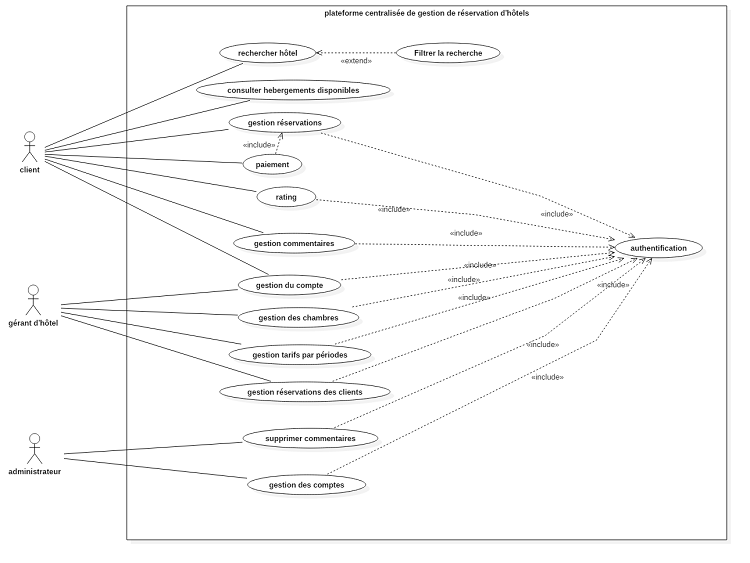
\includegraphics[scale=0.6]{./graphics/usecase.png}
				\caption{Diagramme de cas d'utilisation}
			\end{figure}
			\newpage
		
		\section{Prototype}
Le mock-up, ou dit autrement la maquette fonctionnelle, montre la partie visuelle du projet. Il s’agit d’une représentation statique du contenu, de la structure et des fonctionnalités de l’application.\\
Enfin, le prototype est une maquette interactive. En plus de la partie visuelle, il montre le fonctionnement de l’application. Le prototype est extrêmement utile pour tester la convivialité du projet.\\

			\begin{figure}
			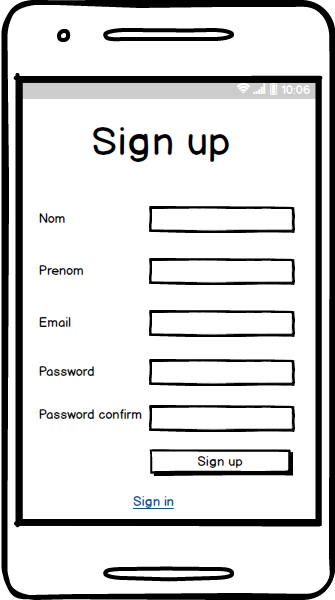
\includegraphics[width=4cm]{./graphics/mk2.png}\hfill
			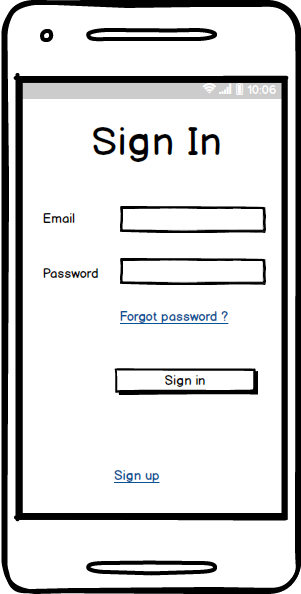
\includegraphics[width=4cm]{./graphics/mk1.png}
			\caption{Maquette création de compte et authentification}
			\end{figure}
			\begin{figure}
			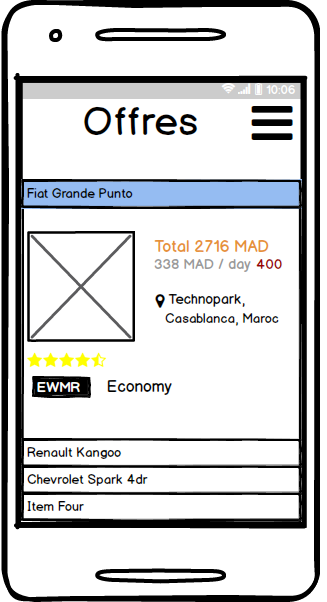
\includegraphics[width=4cm]{./graphics/mk4.png}\hfill
			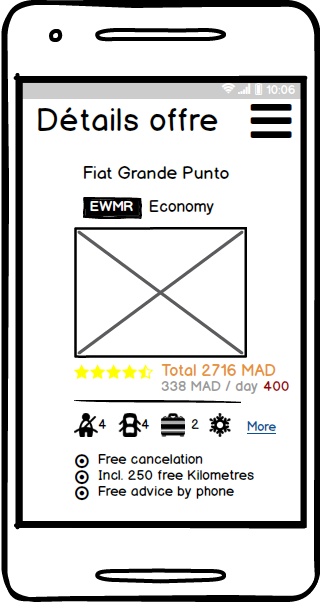
\includegraphics[width=4cm]{./graphics/mk5.png}
			\caption{Maquette offres et détails offre}
			\end{figure}
			\begin{figure}
			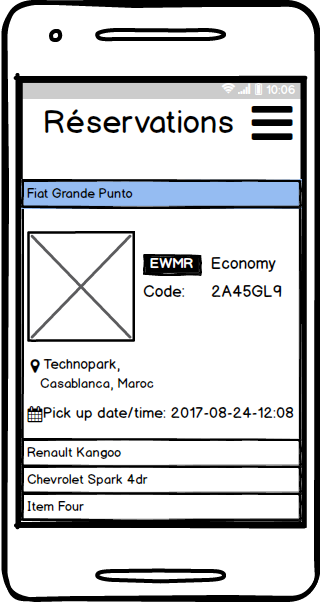
\includegraphics[width=4cm]{./graphics/mk3.png}\hfill
			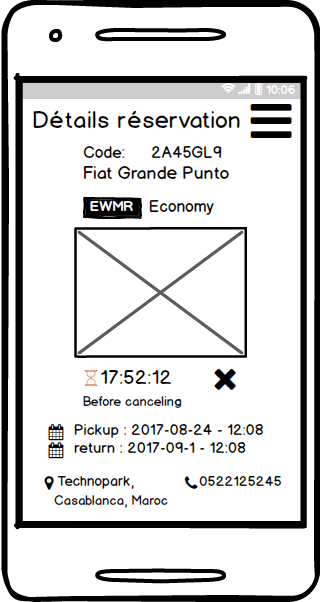
\includegraphics[width=4cm]{./graphics/mk6.png}
			\caption{Maquette réservations et détails réservation}
			\end{figure}
			
			

		%================vue dynamique====================
		\newpage
		~
		\newpage
		\section{Vue Dynamique du système}
			\subsection{Diagramme de séquence:} 
Ces diagrammes sont la représentation graphique des interactions entre les acteurs et le
système selon un ordre chronologique. Ces interactions sont ainsi montrées dans le cadre d'un
scénario d'un diagramme de cas d'utilisation et ils ont pour but de décrire comment se déroule les
actions entre les acteurs ou objets.
			
			\subsection{scénario de réservation de véhicule}
			\vspace{1cm}
			\begin{figure}[!hbtp]
				\centering
				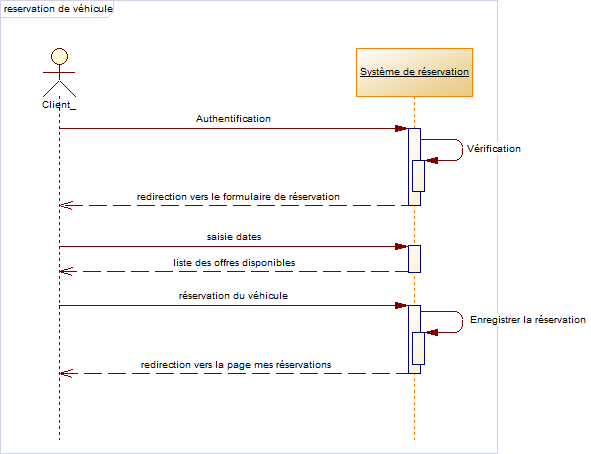
\includegraphics[scale=0.8]{./graphics/sequence.png}
				\caption{Diagramme de séquence}
			\end{figure}

			\newpage
			
		

		%===================mcd===========================
		\section{Modélisation conceptuelle et logique des données}
			\subsection{Modèle Conceptuel des Données}
Le modèle conceptuel des données décrit de façon formelle les données utilisées par le système d’information. Les principales composantes de ce modèle sont des entités et des relations qui peuvent exister entre eux. Il repose sur une représentation graphique (relationnelle) qui facilite considérablement sa compréhension.
			\vspace{2cm}
			\begin{figure}[!hbtp]
				\centering
				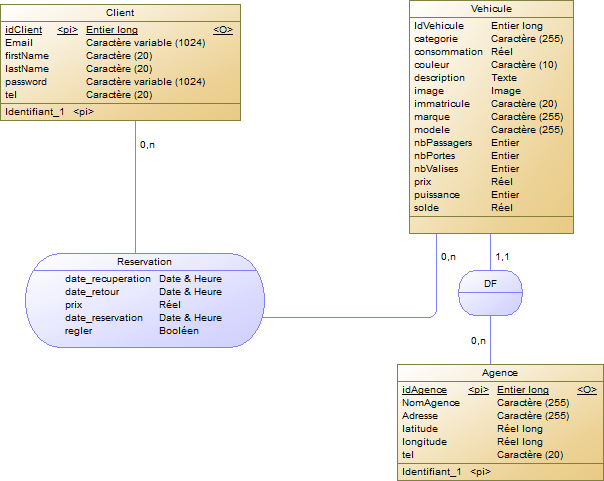
\includegraphics[scale=0.8]{./graphics/mcd.png}
				\caption{Modèle conceptuelle de données}
			\end{figure}
			\newpage
			
			\subsection{Modèle Logique des Données}
Le modèle relationnel représente la base de données comme un ensemble de tables, sans préjuger de la façon dont les informations sont stockées dans la machine. Les tables constituent donc la structure logique du modèle relationnel ou il est possible de relier ces structures à des tables au niveau logique. Les données sont organisées sous forme de relations.
			\begin{figure}[!hbtp]
				\centering
				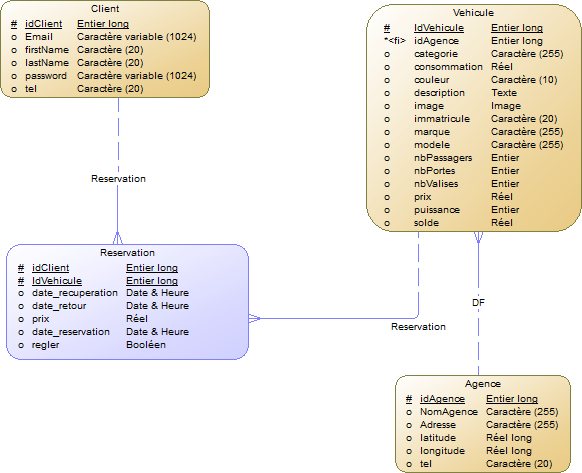
\includegraphics[scale=0.8]{./graphics/mld.png}
				\caption{Modèle logique de données}
			\end{figure}
			
		
		%===========conclusion===========
		\section{Conclusion}
Dans ce chapitre, j'ai présenté l'étude conceptuelle du système. La vue fonctionnelle a été illustrée par un diagramme de cas d’utilisation, la maquette pour définir les zones et les composants de l’interface de l'application, la vue dynamique par un diagramme de séquence qui ma permis d'avoir une vue générale sur le déroulement des cas d'utilisation et leurs exécutions. Enfin, la modélisation conceptuelle et logique des données qui m'a permis de définir la structure du système et de dégager les différentes tables le composant.\\
Dans le chapitre suivant, je détaille quelques aspects de la réalisation.	
	
		















%=========================chapitre 4===========================
		\chapter{Conception technique}
		

		%=========intro==============
		\section{Introduction}
Il s’agit dans ce chapitre d’identifier les différentes caractéristiques de l’environnement logiciel ainsi que les technologies qui nous ont servi à l’implémentation de notre application.		
		
		
		%=========Plateforme ScreenDy===========
		\section{Plateforme ScreenDy}
Il s'agit d'un environnement de développement visuel qui facilite et accélère la création d'une interface utilisateur mobile, la définition de services de flux, le mappage des services vers l'interface utilisateur et même le test de l'application. Cependant, on n'est pas limité par le constructeur visuel. On peut utiliser nos éditeurs de code ou n'importe quel code JavaScript, HTML5 ou CSS personnalisé pour créer toutes les fonctionnalités que nous voulons.\\
L'application finale est NATIVE et peut être facilement installé sur l'appareil.\\
Cépendant la plateforme est toujours en version Beta, donc instable et peut-on résulter plusieurs bugs.

		\subsection{Création des vues sur ScreenDy}
Sur la plateforme ScreenDy, la création de template est devenue beaucoup plus facile. Elle nous offre tous les composants dont nous avons besoin. On peut obtenir un beau modèle adapté aux différents appareils.\\
Une template est un moyen de séparer le contenu de la forme (comment il est présenté). Cela dit, il agit comme une structure dans laquelle seuls certains éléments sont modifiables (contenu et style).
		
		
		\begin{figure}[!hbtp]
			\centering
			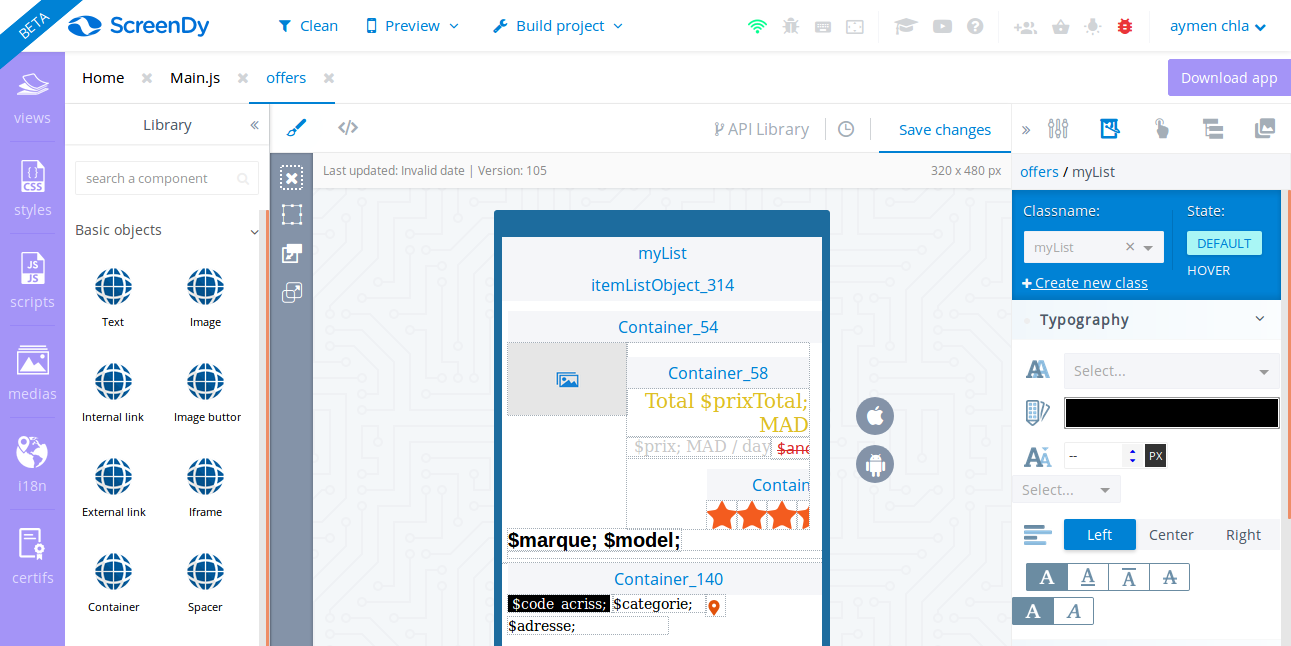
\includegraphics[scale=0.3]{./graphics/vue_screendy.png}
			\caption{Création de vues sur ScreenDy}
		\end{figure}
		\newpage

	
			\subsubsection{\'Etapes générales}
Le schéma suivant présente le cycle de vie de la création de template sur la plate-forme ScreenDy.
Dans les trois premières étapes, nous utilisons un logiciel de désign et outil de prototypage.\\
		
			\begin{itemize}
				\item \textbf{Prototype:} Avant de commencer à créer notre design, il est préférable de dessiner un prototype en utilisant un logiciel de prototypage afin d'avoir une idée générale de notre désign (Balzamiq, Fluid Ui, etc.).
				\item \textbf{Désign:} Dans cette étape, nous définissons à quoi ressemble notre template, en utilisant n'importe quel logiciel de désign (Photoshop,Sketch,etc.).
				\item \textbf{Découpage:} On sépare chaque composant de notre désign et on l'enregistre.
				\item \textbf{Importation des médias:} On télécharge tous les éléments dans la librairie médias.
				\item \textbf{Style:} Après avoir le bon format de notre template, on ajoute du style CSS.
				\item \textbf{Test:} On lance le projet sur l'émulateur pour voir les résultats de notre travail dans différentes appreils.
				\item \textbf{Exportation:} On exporte la template pour l'utiliser dans notre application.
			\end{itemize}
		
		
			\begin{figure}[!hbtp]
				\centering
				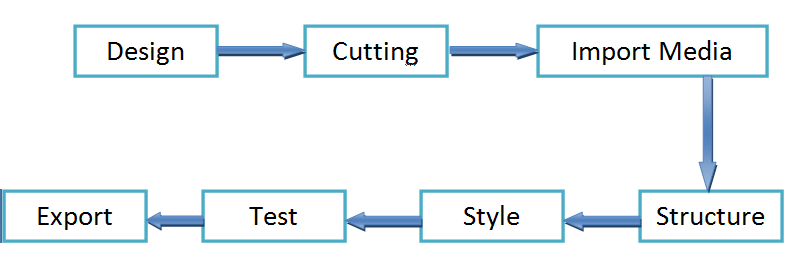
\includegraphics[scale=0.5]{./graphics/general-steps.png}
				\caption{\'Etapes génarales}
			\end{figure}	

			\newpage


		\subsection{Ajout des fonctions Javascript}
Une fois on crée vos vues sur la plateforme ScreenDy, On doit ajouter le traitement Javascript pour les fonctionnalités de notre application.
			\begin{figure}[!hbtp]
			\centering
			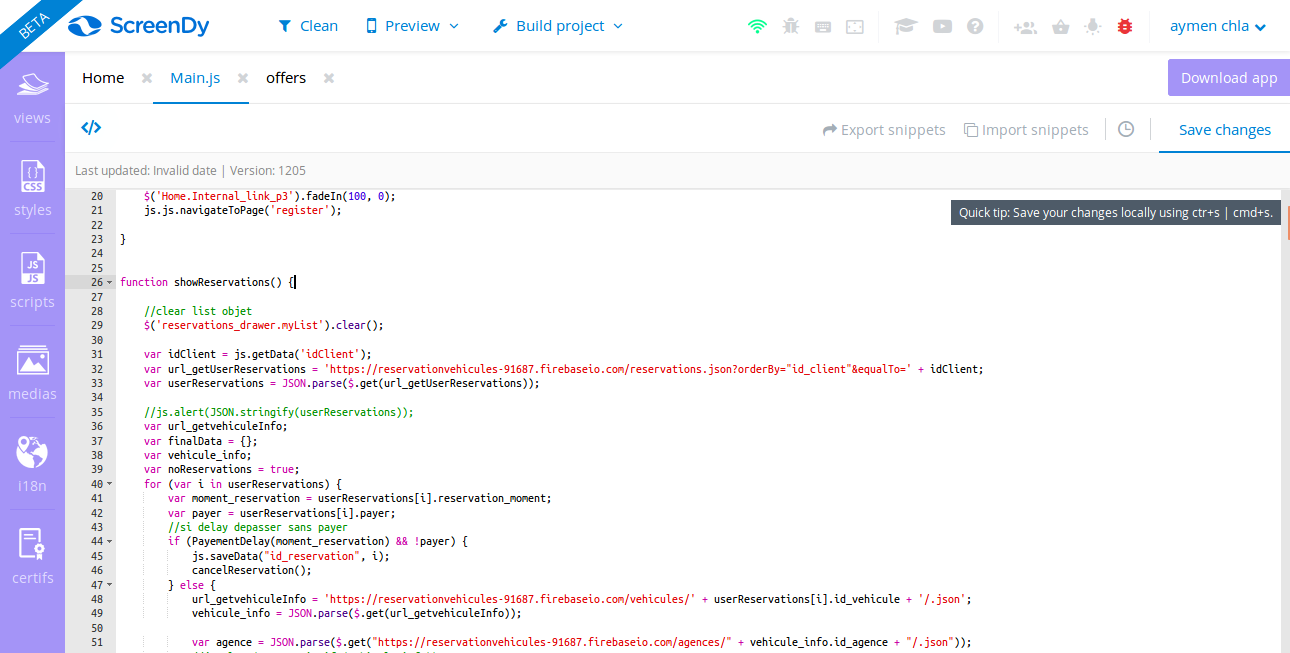
\includegraphics[scale=0.3]{./graphics/js_screendy.png}
			\caption{Traitement JavaScript sur ScreenDy}
			\end{figure}

			\subsubsection{ScreenDy JavaScript}
			\begin{wrapfigure} {r}{3cm}
			
\includegraphics[scale=0.5]{./graphics/js.png}
			\end{wrapfigure}

ScreenDy JavaScript Est un langage qui nous permet d'ajouter des fonctionnalités et de développer natif. La transformation utilisée par screendy pour passer de javascript à java / Objective-C ne supportera pas toutes les variables telles que window, document, console ... ces variables sont remplacées par des variables équivalentes dans le même objet widget, page, log ...\\
Screendy implémente le JavaScript car c'est un langage haut niveau, dynamique, non typé, etc. Parallèlement à HTML et CSS, il est l'une des trois technologies de base de la production World Wide Web. C'est un langage rapide et concis qui simplifie le déplacement de documents HTML, la gestion des événements, l'animation et les interactions pour un développement web rapide.\\
La syntaxe Javascript, la déclaration de fonction (fonction), la déclaration de variable (var) et toutes les méthodes indépendantes de DOM sont communes entre JavaScript ScreenDy et JavaScript Classic.



		\subsection{Test de l'application}
			\subsubsection{Sur smartphone}
Pour ce faire on doit télécharger depuis le Play Store l'application "ScreenDy previewer" et l'installer sur notre device, une fois fait,  on ouvre l'application et on accède au contenu avec le même compte que nous avons créé sur la plateforme. Il suffit par la suite de cliquer sur le nom de l'application affiché et elle sera exécutée.
			\subsubsection{Sur l'émulateur}
L'émulateur de la plateforme nous donne la possibilité de voir les résultats de l'application sur les deux Systèmes d'exploitation (Android et IOS) et sur différentes tailles d'écrans.
			\begin{figure}[!hbtp]
			\centering
			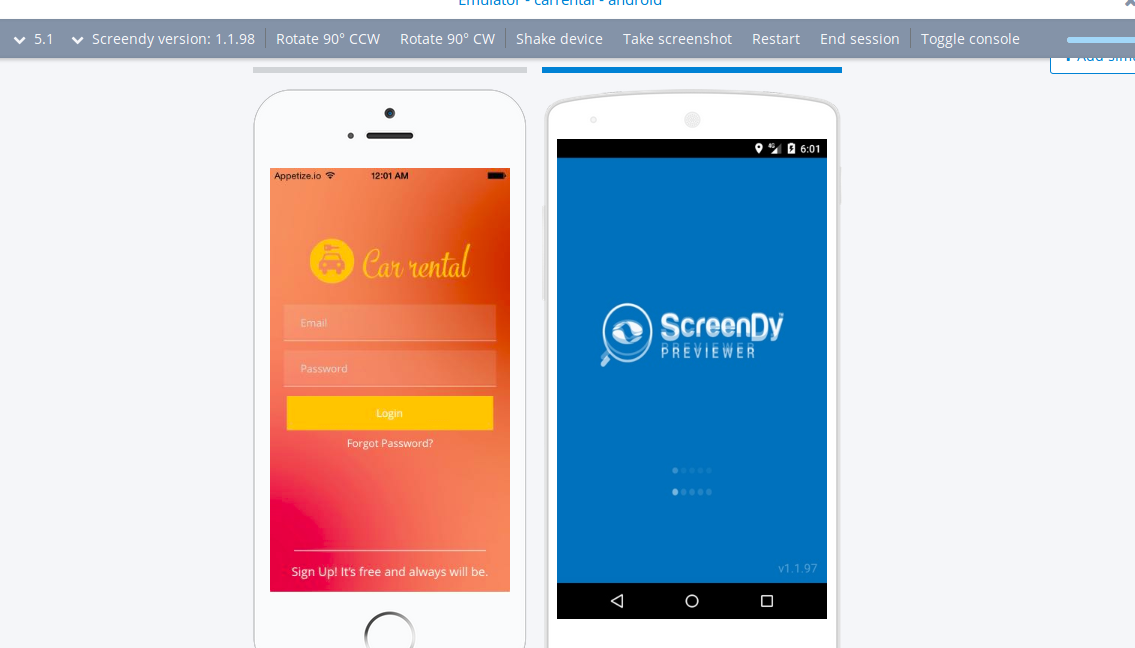
\includegraphics[scale=0.3]{./graphics/emul.png}
			\caption{Test sur l'émulateur de ScreenDy}
			\end{figure}

		%==============fin section screendy==============

		\newpage

		%==============Firebase==========================
		\section{Firebase}
		\begin{wrapfigure} {r}{3cm}
		
\includegraphics[scale=0.15]{./graphics/firebase.png}
		\end{wrapfigure}
Firebase est un ensemble de services d'hébergement pour n'importe quel type d'application (Android, iOS, Javascript, Node.js, Java, Unity, PHP, C++ ...). Il propose d'héberger en NoSQL et en temps réel des bases de données, du contenu, de l'authentification sociale (Google, Facebook, Twitter et Github), et des notifications, ou encore des services, tel que par exemple un serveur de communication temps réel. Lancé en 2011 sous le nom d'Envolve, par Andrew Lee et par James Templin, le service est racheté par Google en octobre 2014. Il appartient aujourd'hui à la maison mère de Google : Alphabet.\\
Firebase donne la possibilité de communiqué avec la base donnée en utilisant le REST API avec du format JSON.


		%===========rest api==========================
		\section{REST API}
		\begin{wrapfigure} {r}{3cm}
		
\includegraphics[scale=0.2]{./graphics/logo_restapi.png}
		\end{wrapfigure}
REST est une architecture de services Web. Élaborée en l'an 2000 par Roy Fiedling, l'un des
créateurs du protocole HTTP, du serveur Apache HTTPd et d'autres travaux fondamentaux, REST
est une manière de construire une application pour les systèmes distribués comme le World Wide
Web.\\
Une API compatible REST, ou \guillemotleft RESTful \guillemotright, est une interface de programmation d'application qui fait appel à des requêtes HTTP pour obtenir (GET), placer (PUT), publier (POST) et supprimer (DELETE) des données.\\
Ce web service support le format XML et le format JSON.
		\begin{figure}[!hbtp]
		\centering
		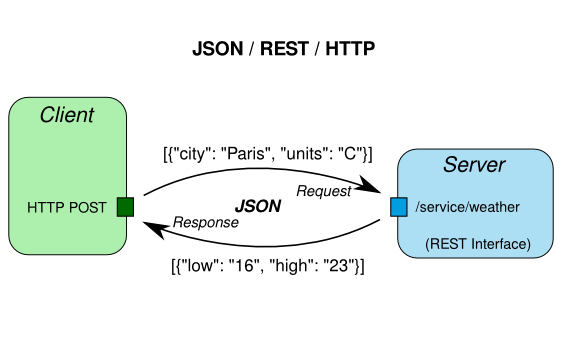
\includegraphics[scale=0.5]{./graphics/restapi.png}
		\caption{Schéma REST API}
		\end{figure}
		

		\newpage	

		%================JSON==========================
		\section{JSON}
		\begin{wrapfigure} {r}{3cm}
		
\includegraphics[scale=0.3]{./graphics/json.png}
		\end{wrapfigure}
JSON est un format de données textuelles dérivé de la notation des objets du
langage JavaScript. Il permet de représenter de l’information structurée comme le permet XML par
exemple. Créé par Douglas Crockford entre 2002 et 2005.\\
Un document JSON a pour fonction de représenter de l'information accompagnée d'étiquettes
permettant d'en interpréter les divers éléments, sans aucune restriction sur le nombre de celles-ci.
		
		\section{Git et Github}
		\begin{wrapfigure} {r}{3cm}
		
\includegraphics[scale=0.25]{./graphics/gitgithub.jpg}
		\end{wrapfigure}
		Git est un système de contrôle de version (VCS) pour suivre les changements dans les fichiers et coordonner le travail sur ces fichiers entre plusieurs personnes. Il est principalement utilisé pour le développement de logiciels, mais il peut être utilisé pour garder une trace des changements dans les fichiers.\\
Github est un service web d'hébergement et de gestion de développement logiciel utilisant les logiciels de gestion de versions Git.

		\section{Conclusion}
Au cours de ce chapitre, J'ai présenté l’environnement de développement et les différents outils utilisés pour la mise en place de l’application.

%===============================fin chapitre conception conception technique===================












%================================chapitre Réalisation==============================
	\chapter{Réalisation}

	\section{Introduction}
La phase qui suit une conception bien détaillée est éventuellement l’implémentation. Le module additionnel sera implémenté en tant qu’une application mobile répondant à plusieurs exigences. En effet, le projet devrait être développé sous la plateforme ScreenDy en utilisant la base de données existante Firebase.

	\section{Application mobile pour la réservation de véhicules}
	\subsection{Interfaces}
Les figures ci-dessous représentent quelques captures d’écran de pages de mon application. Les pages qui suivent l’authentification contiennent tous un menu, qui va nous permettre de naviguer dans les différentes pages de l'application.\\
Dans cette partie je vais décrire la réalisation sous forme d’un scénario de réservation de véhicule.
	\newpage
	\subsubsection{Page d'accueil}
Cette page donne une idée générale sur le fonctionnement de l'application.
	\vspace{2cm}
	\begin{figure}[!hbtp]
		\centering
		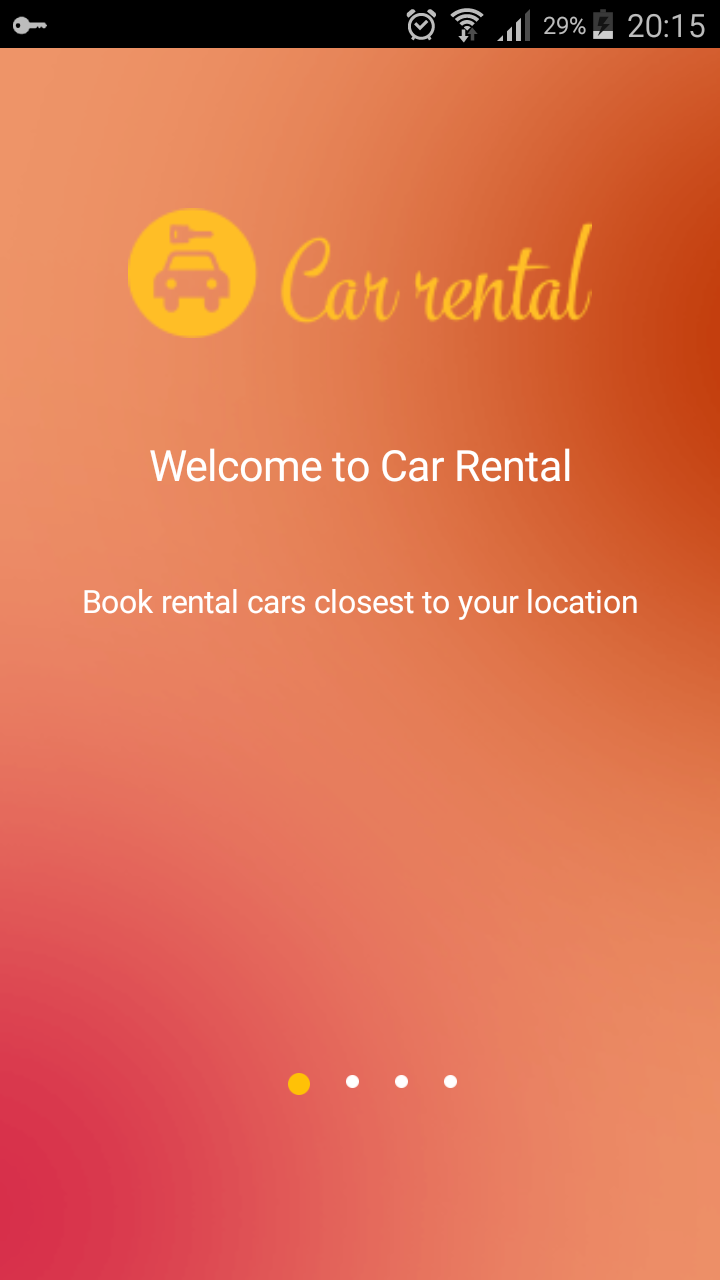
\includegraphics[scale=0.2]{./graphics/Accueil.png}
		\caption{Page d'accueil}
		\end{figure}
		\newpage

	\subsubsection{Menu de navigation}
Le menu permet de naviguer dans les différentes pages de l'application.
	\vspace{2cm}
	\begin{figure}[!hbtp]
		\centering
		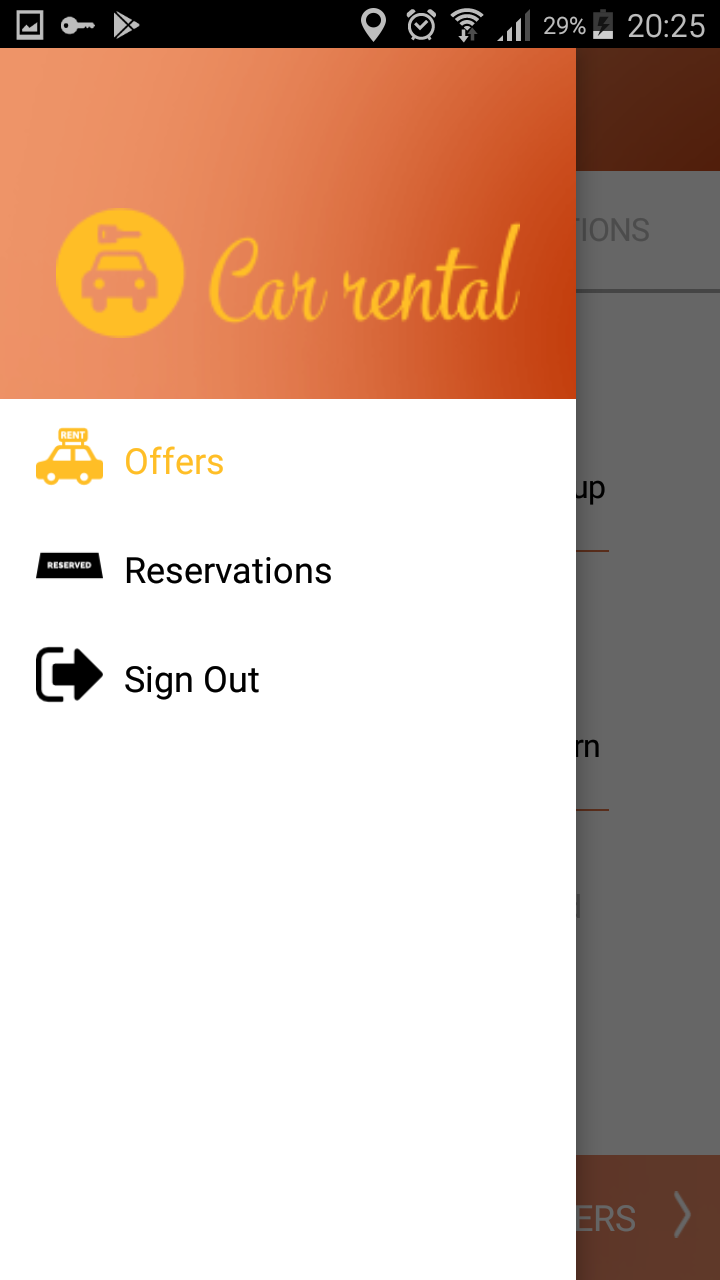
\includegraphics[scale=0.2]{./graphics/Menu.png}
		\caption{Menu de navigation}
		\end{figure}
		\newpage

	\subsubsection{Création d'un nouveau compte}
Cette interface permet au client de créer son propre compte en saisissant ses informations.
	\vspace{2cm}
	\begin{figure}[!hbtp]
		\centering
		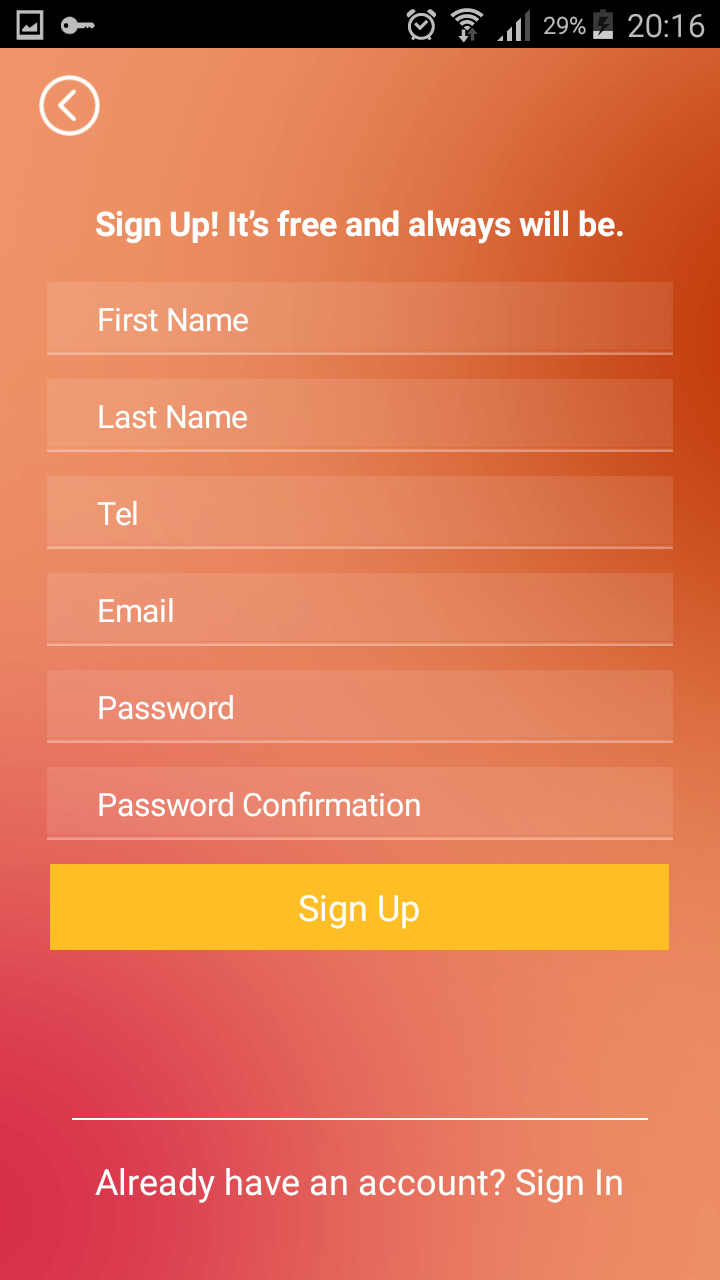
\includegraphics[scale=0.2]{./graphics/Signup.png}
		\caption{Création d'un nouveau compte}
		\end{figure}
		\newpage

	\subsubsection{Authentification}
Afin d’avoir accès à l’ensemble des fonctionnalités offertes par l’application, l’utilisateur doit
saisir son email et son mot de passe valides.
	\vspace{2cm}
	\begin{figure}[!hbtp]
		\centering
		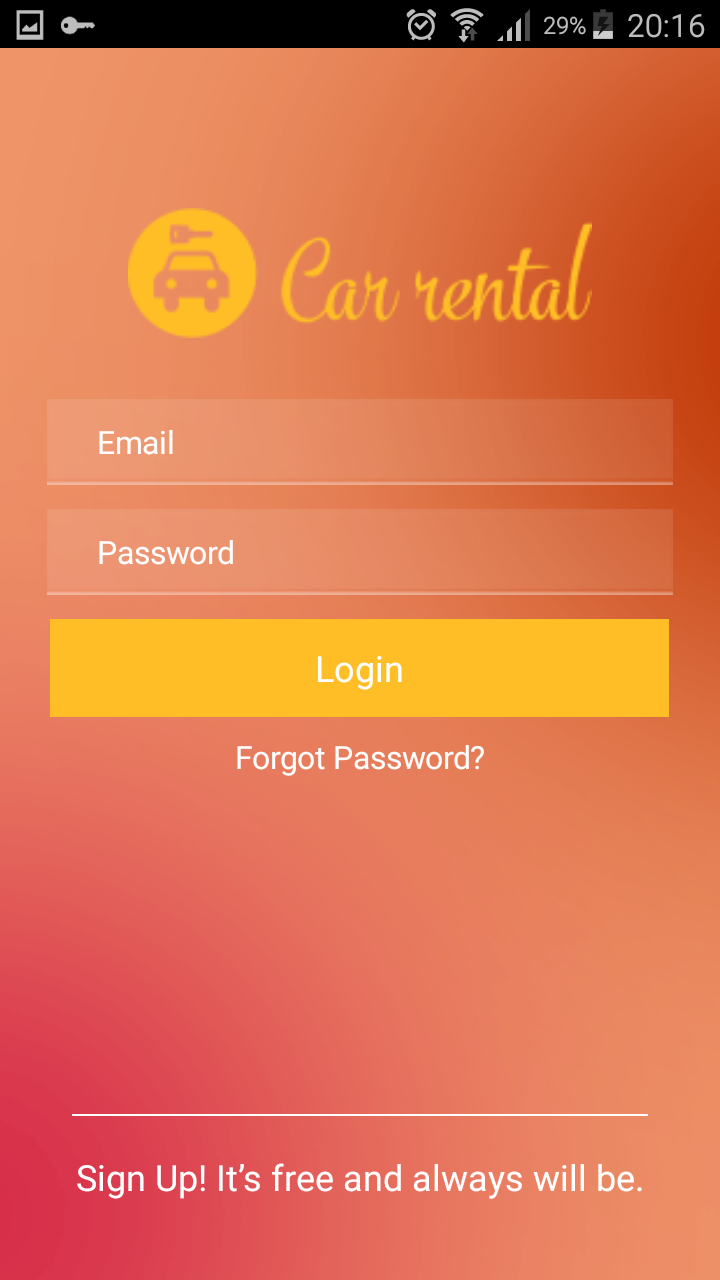
\includegraphics[scale=0.2]{./graphics/Signin.png}
		\caption{Authentification}
		\end{figure}
		\newpage
	
	\subsubsection{Recherche des offres}
Cette interface permet au client de chercher les offres disponibles durant la période choisie.
	\vspace{2cm}
	\begin{figure}[!hbtp]
		\centering
		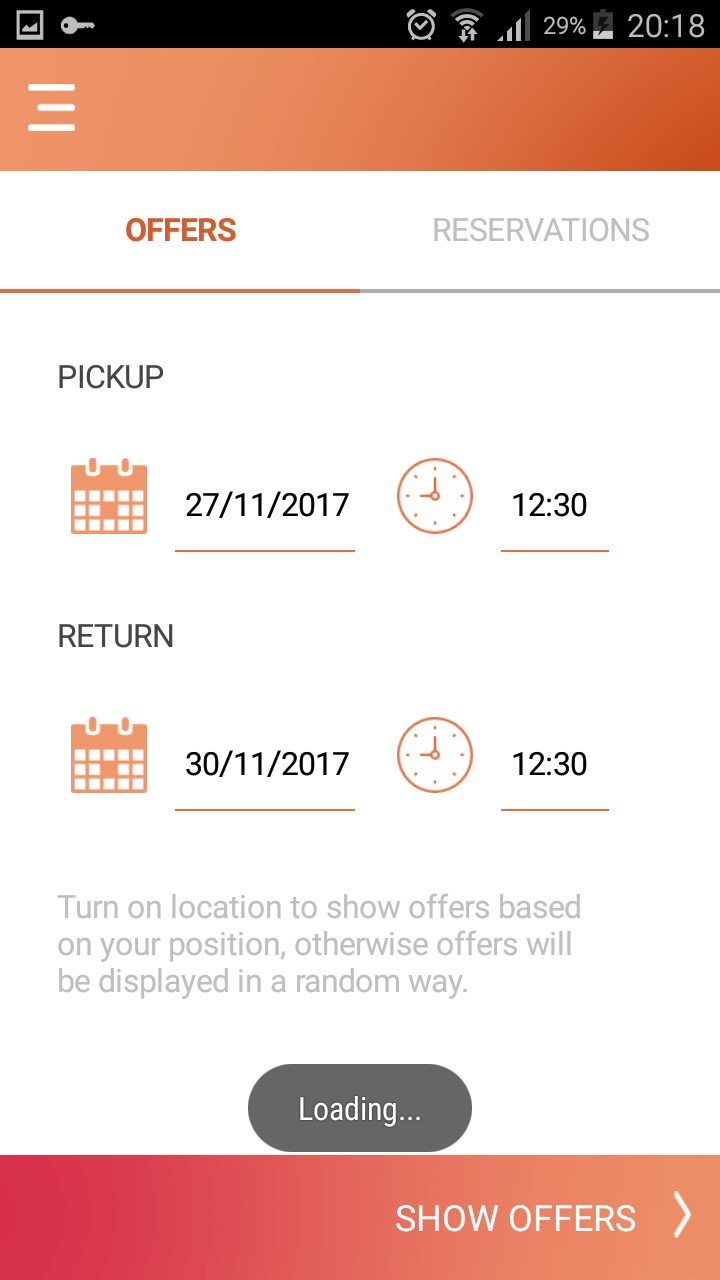
\includegraphics[scale=0.2]{./graphics/Date.png}
		\caption{Recherche des offres}
		\end{figure}
		\newpage

	\subsubsection{Consultation des offres}
Cette interface affiche la liste des offres disponible pour la réservation durant la période choisie.
	\vspace{2cm}
	\begin{figure}[!hbtp]
		\centering
		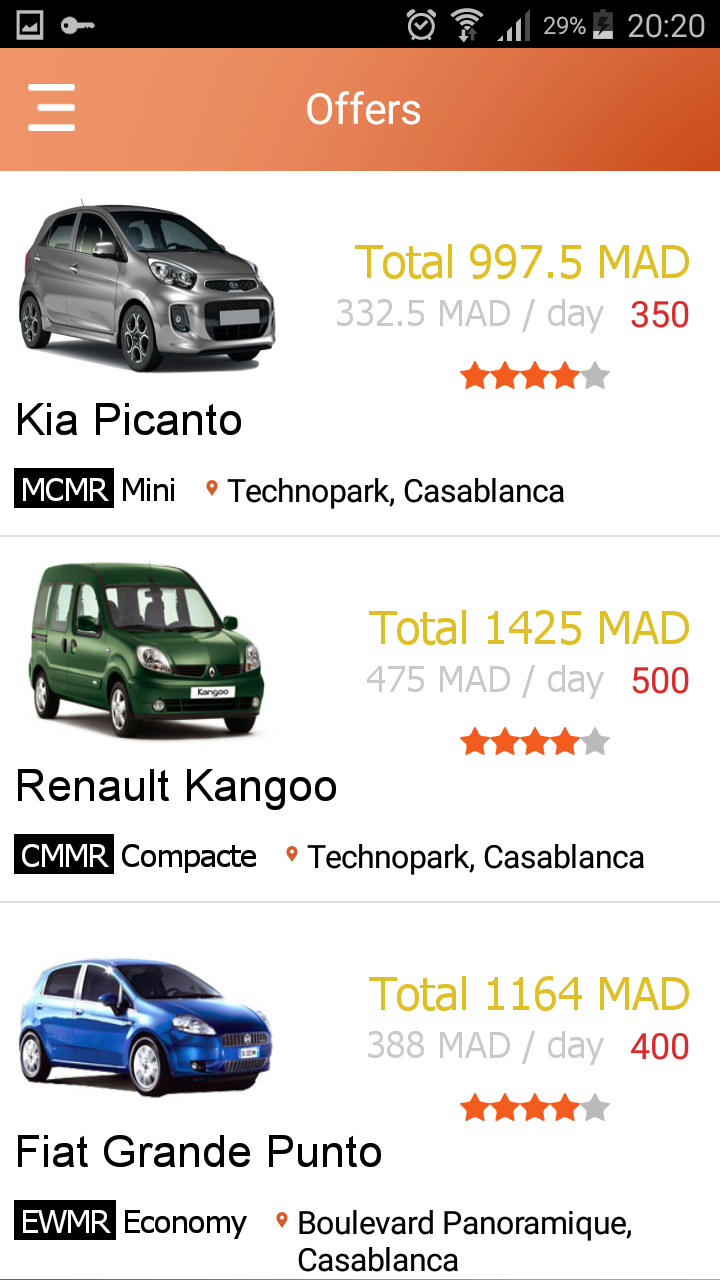
\includegraphics[scale=0.2]{./graphics/Offres.png}
		\caption{Offres}
		\end{figure}
		\newpage		
	
	\subsubsection{Consultation des détails}
Cette interface affiche les détails de l'offre choisie elle permet aussi de le réserver.
	\vspace{2cm}
	\begin{figure}[!hbtp]
		\centering
		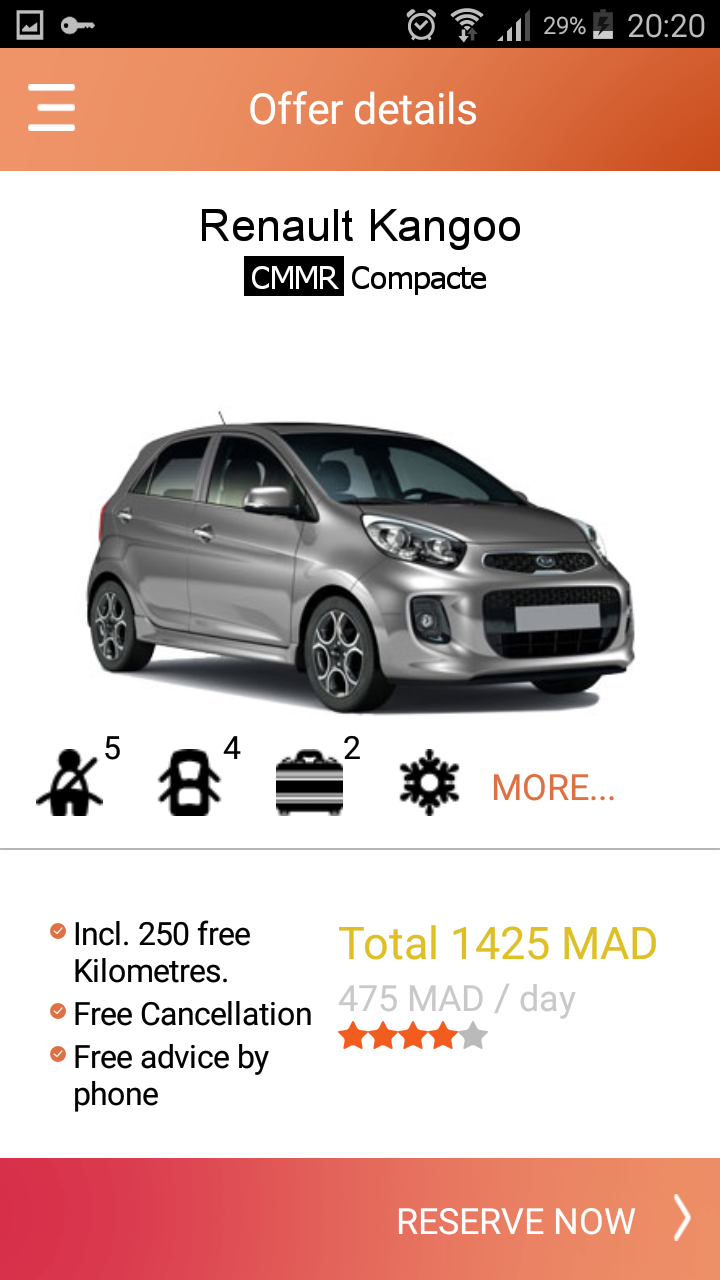
\includegraphics[scale=0.2]{./graphics/DetailsOffre.png}
		\caption{Détails offre}
		\end{figure}
		\newpage

	\subsubsection{Consultation des condition de réservations}
	\vspace{2cm}
	\begin{figure}[!hbtp]
		\centering
		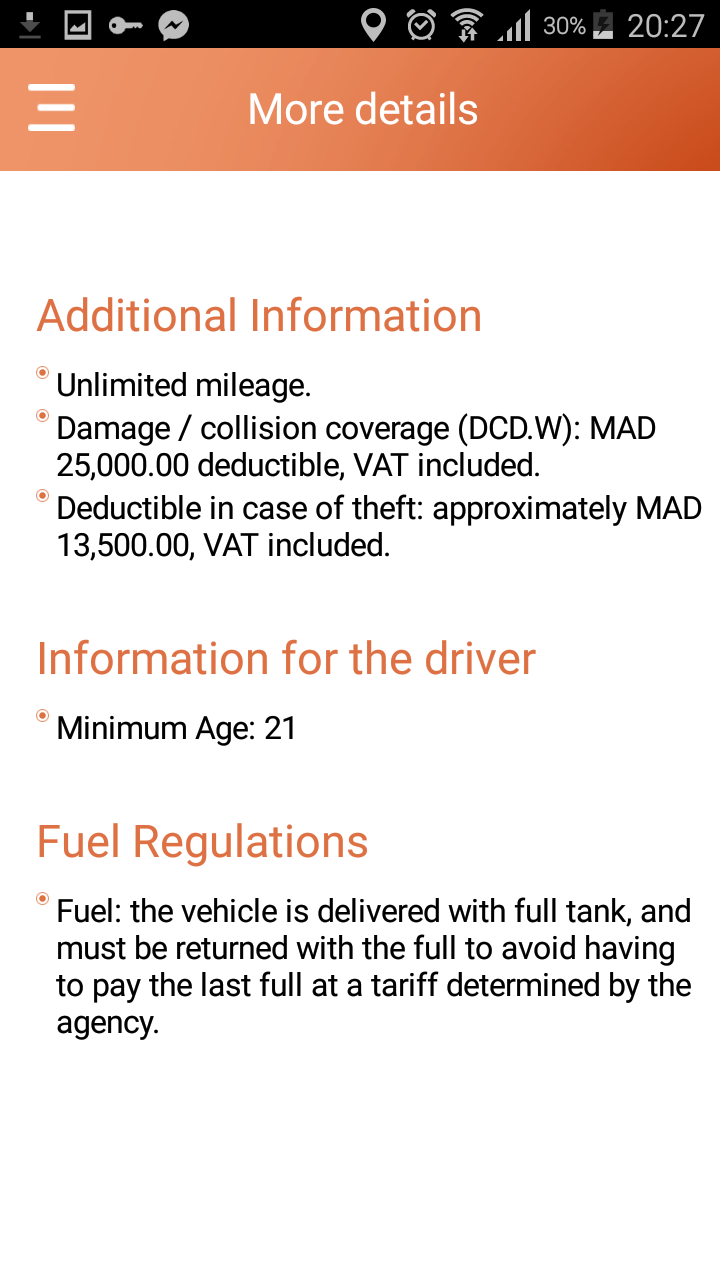
\includegraphics[scale=0.2]{./graphics/More.png}
		\caption{Conditions}
		\end{figure}
		\newpage
	
	\subsubsection{Consulter ses réservations}
Cette interface affiche la liste des réservations du client
	\vspace{2cm}
	\begin{figure}[!hbtp]
		\centering
		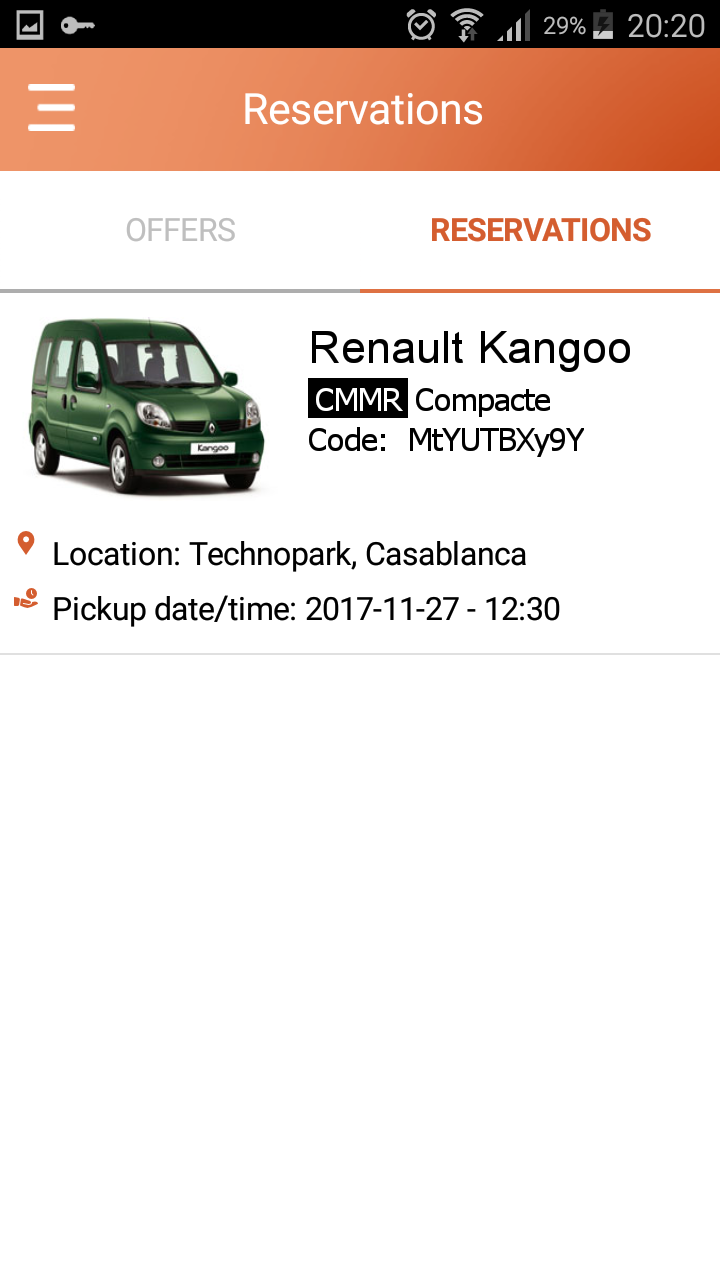
\includegraphics[scale=0.2]{./graphics/Reservations.png}
		\caption{Réservations}
		\end{figure}
		\newpage

	\subsubsection{Consulter détails réservations}
Cette interface affiche les détails de la réservation à savoir le code, la date et le lieu de la réservation ainsi que la durée restante avant l'annulation au cas où la réservation n'est pas encore confirmé.
	\vspace{2cm}
	\begin{figure}[!hbtp]
		\centering
		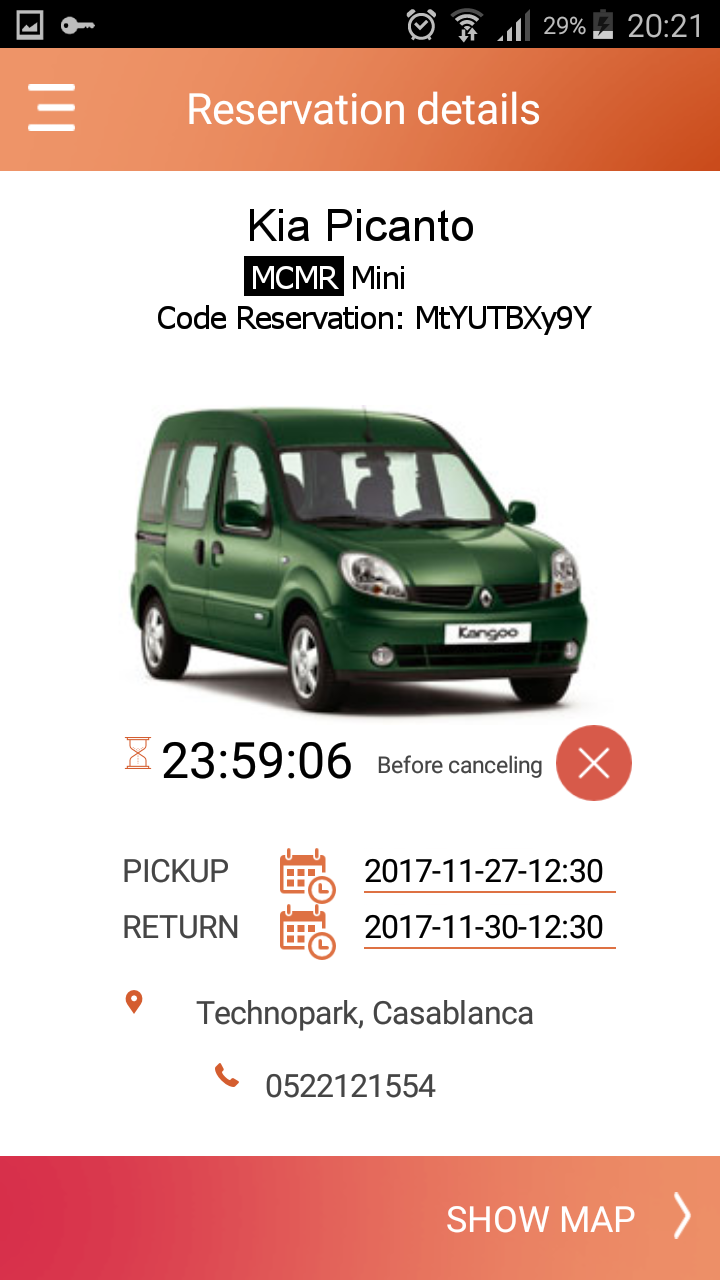
\includegraphics[scale=0.2]{./graphics/DetailsReservation.png}
		\caption{Détails réservation}
		\end{figure}
	
	 \section{APIs}
La 2\up{ème} phase du stage consiste à utiliser des APIs sur des applications ScreenDy.\\
Pour ce faire il faut faire une recherche dans la documentation officielle des fournisseurs mentionnés par l'encadrante. Une fois intéressé à un fournisseur il faut choisir les API (web service Rest) à traité.
Les APIs choisis sont:\\
	\begin{itemize}
		\item Recherche de place de Facebook
		\item Extraction de profile d'Instagram
	\end{itemize}

	

	\begin{figure}
	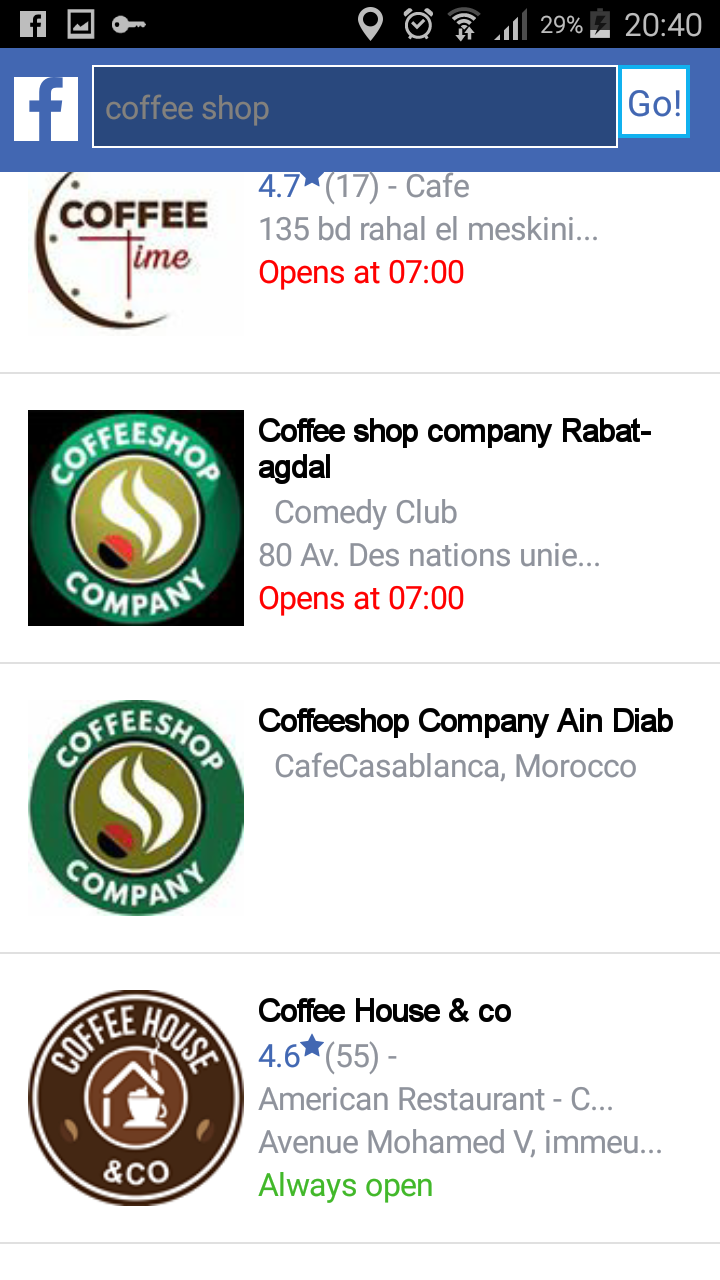
\includegraphics[width=5cm]{./graphics/fb.png}\hfill
	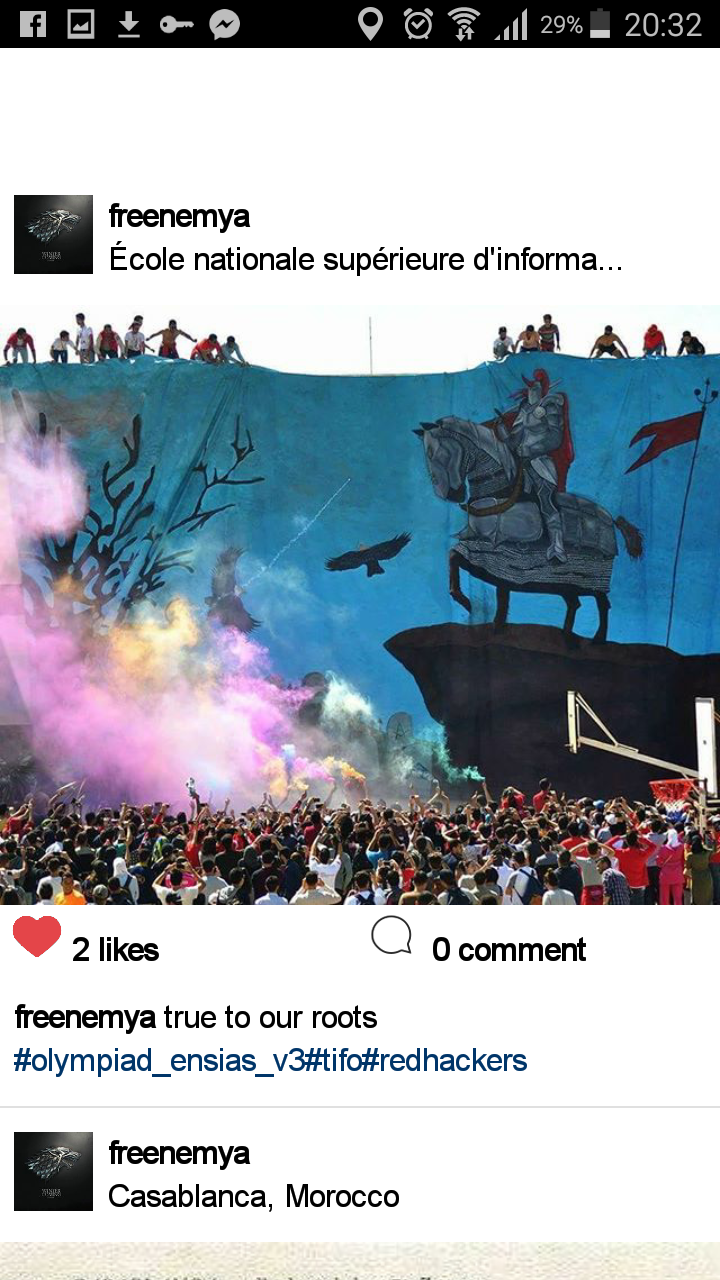
\includegraphics[width=5cm]{./graphics/instagram.png}
	\caption{APIs}
	\end{figure}
				
	\section{Conclusion}
Au cours de ce chapitre, j'ai présenté la dernière étape du développement, qui est
celle de la réalisation et de la mise en œuvre du projet. J'ai présenté le résultat de la fusion
de tous les éléments de spécifications fonctionnelles et techniques précédemment traitées.
%====================================fin réalisation=================================




%=================================conclusion générale==========================

		\chapter*{Conclusion générale} 
	\addcontentsline{toc}{chapter}{Conclusion}
	Ce stage de fin de 1\up{ère} année avait pour but majeur la solidification et la mise en
pratique de l’ensemble des compétences théoriques et techniques acquises durant l’année scolaire. Il
consistait à travailler sur une application mobile pour automatiser le processus de réservation des véhicules pour donner au client un service confortable.\\
Malgré la limite du temps réservé à la réalisation de ce projet qui demeure pour moi un projet
de taille et complexité assez importantes et les difficultées que j'ai rencontrés lors de la phase de réalisation que ça soit les bugs de la plateforme qu'est toujours en version Beta ainsi que l'inexistance de communauté pour le partage de solution, j'ai pu concrétiser les objectifs tracés initialement, dans les délais estimés. Au début, j'ai commencé à exprimer les exigences et les besoins de l’organisme, puis après la validation du cahier des charges j'ai passé aux
spécifications techniques et fonctionnelles. Après validation de ces spécifications avec le chef de
projet, je me suis mis à développer l'application.\\
Effectivement l'application n'est pas parfaite et beaucoup de choses peuvent être ajoutées ou bien modifiées.\\
En matière de ce projet, j'ai eu l’opportunité d’acquérir de nouveaux concepts, dont les principaux sont le développement d'applications sous la plateforme ScreenDy et de travailler avec un nouveau type de SGBD qu'est le NoSQL, ce qui est vraiment intéressant pour les prochains
projets.\\
	
	\chapter*{Bibliographie}
	\addcontentsline{toc}{chapter}{Webographie}
	\bibliographystyle{plain}
	\vspace{2cm}
	  \begin{itemize}
	 		\item http://docs.screendy.com/
			\item https://firebase.google.com/docs/reference/rest/database/
			\item https://fr.wikipedia.org/wiki/Classification\_ACRISS
			\item https://developers.facebook.com/docs/places/web/search/
			\item https://www.instagram.com/developer/endpoints/media/
			\item https://fr.wikipedia.org/wiki/Representational\_state\_transfer
			\item https://fr.wikipedia.org/wiki/JavaScript\_Object\_Notation
		\end{itemize}
	\end{document}
